% define document type, font-size, and paper dimensions
\documentclass[11pt, letterpaper]{article}
% set up image package & path
\usepackage{graphicx}
% subcaption for multi-figures
\usepackage{subcaption}
% adds a header onto every page
\usepackage{fancyhdr}
% adds indent to paragraph after section header
\usepackage{indentfirst}
% make margins 1in
\usepackage[total={6.5in,8.75in},
top=1.25in, left=1in]{geometry}
% add hyperlinks
\usepackage{hyperref}
% adjusting figures
\usepackage{float}

% set up page style & graphic path
\pagestyle{fancy}
\graphicspath{{./images/}}

% Resize table rows
\renewcommand{\arraystretch}{1.75}

% Set up title page
\renewcommand{\maketitle}{
    \begin{titlepage}
        % Set up title page
        \centering
        \huge{\textbf{ECS 171 Group 10 Project}} \par
        \vspace{.5cm}
        % group leader
        \large{Leader: Ryan Yu} \par
        \vspace{.5cm}
        % group members
        \normalfont{Amira Basyouni, Calvin Chen, Alexis Lydon, Tianming Tan} \par
        \vspace{.5cm}
        % github repo
        \normalfont{Github Repository: \url{https://github.com/ryyu444/ECS-171-Group-Project} \par}
        \vspace{.5cm}
        % date
        \today
    \end{titlepage}
}

% set up header
\fancyhf{} % clear all header and footer fields
\lhead{The Effects of Sleep} % left header
\rhead{\thepage} % right header
%\fancyhfoffset[LR]{1cm} % increase left, right margin by 1cm

\begin{document}
    \maketitle
    
    \newpage

    \section*{Introduction and Background}
    As a student, we constantly grapple with numerous stressors while striving for academic success. Deadlines, exams, and the intrinsic self-asserted pressure to excel, they all contribute to the challenges we face. These factors can have a negative impact on our quality of learning, hindering our progress toward acquiring a degree and entering the workforce. In contrast, sleep is an activity that we all partake in and is seemingly a relaxant for many. So, we posed a question: does sleep have connections to stress? And if so, what is the relationship between them? For our goals, we would like to predict the effects that sleep quality and sleep duration can have on our stress levels. After we analyze our data, we will be able to determine the correlation between stress and those two attributes. It’s worth noting that our data includes individuals aged 27 to 59. Although the range does not cover the typical college student age, our results can still provide valuable insights for building awareness that can benefit us in the years to come.

    In this machine learning project centered on the intersection of sleep health and stress, our primary objective is to examine the correlation between key attributes such as sleep duration and sleep quality, and their influence on stress levels. This analysis will help us better understand and predict the dynamics between these factors and identify the attributes that have the most significant impact on stress levels. As an integral part of the project, we will develop accurate models for stress prediction based on the highly correlated attributes in our dataset. 


    \section*{Literature Review}
    Machine Learning has great capabilities within the realm of pattern recognition and categorization, two fields that we hope to utilize as we explore the connection between sleep and stress. It is important to address some of the pre-existing studies which were conducted with a similar objective. Presented below are examples of such research and methodologies as well as their overall findings.
    
    Jayawickrama and Rupasingha, researchers from Sabaragamuwa University of Sri Lanka, conducted a study to examine the impact of sleep habits on stress levels. (1) They applied various machine learning models, including Naïve Bayes, Random Forest, Decision Trees, Multi-layer Perceptrons (MLPs), Support Vector Machines (SVMs), and Logistic Regression mixed with cross-validation. It was revealed that five of the six models achieved accuracy rates exceeding 80%, suggesting that there is a strong correlation between sleep and stress. Notably, Naïve Bayes was the best predictor with an accuracy of 91.27%. 
    
    Minhazur Rahman and a different group of researchers predicted stress levels using data collected from sleeping participants. (2) Some of the models they utilized include Gradient Boosting, Decision Trees, Random Forest, Gaussian Naive Bayes, and Linear Support Vector Machine. Their models achieved an accuracy rate of over 95\%, with Naive Bayes and SVM as the top performers. 
    
    Overall, these studies highlight the efficacy of machine learning models in predicting stress levels based on sleep data, with Naive Bayes and SVM demonstrating high performance. We hope to utilize these research metrics as the basis of judgment for the models that we will be building and testing.
    

    \section*{Dataset Description and Exploratory Data Analysis}
    The dataset being used in this project is the “Sleep Health and Lifestyle Dataset” by Laksika Tharmalingam, accessible on Kaggle. The dataset comes in the form of a CSV file and contains 400 rows and 13 columns, consisting of various sleep and lifestyle variables–gender, age, occupation, sleep duration, sleep quality, and stress levels for example. These variables encompass the very aspects of sleep and health that can be useful in predicting stress. Despite the abundant source of data, a limitation of this dataset is its synthetic nature, generated artificially rather than from real-world observations. Although it may lack certain real-world nuances, high-quality synthetic data proves effective in emulating real datasets. It serves as a cost-efficient and time-saving alternative for gathering real-world observations to use for training and testing machine learning models.
    
    Initially, we conducted essential data preprocessing to convert all categorical data into numerical values, enhancing their compatibility with prediction models. This involved applying label encoding to categorical attributes from the dataset, like BMI and Gender in the dataset. We opted for label encoding over one-hot encoding to maintain consistency in the number of columns in our dataset and to enhance clarity in visualization such as the pair plot and correlation matrix. 
    
    Following data preprocessing, we generated a pair plot matrix (reference to figure) to identify potential linearly separable relationships between attributes and Stress Level. The pair plot revealed notable linear associations, particularly between Sleep Quality and both Sleep Duration and Age in predicting Stress Level. Additionally, Sleep Duration and Gender also have somewhat of a linear relationship in predicting stress. 

    \begin{figure}[H]
        \centering
        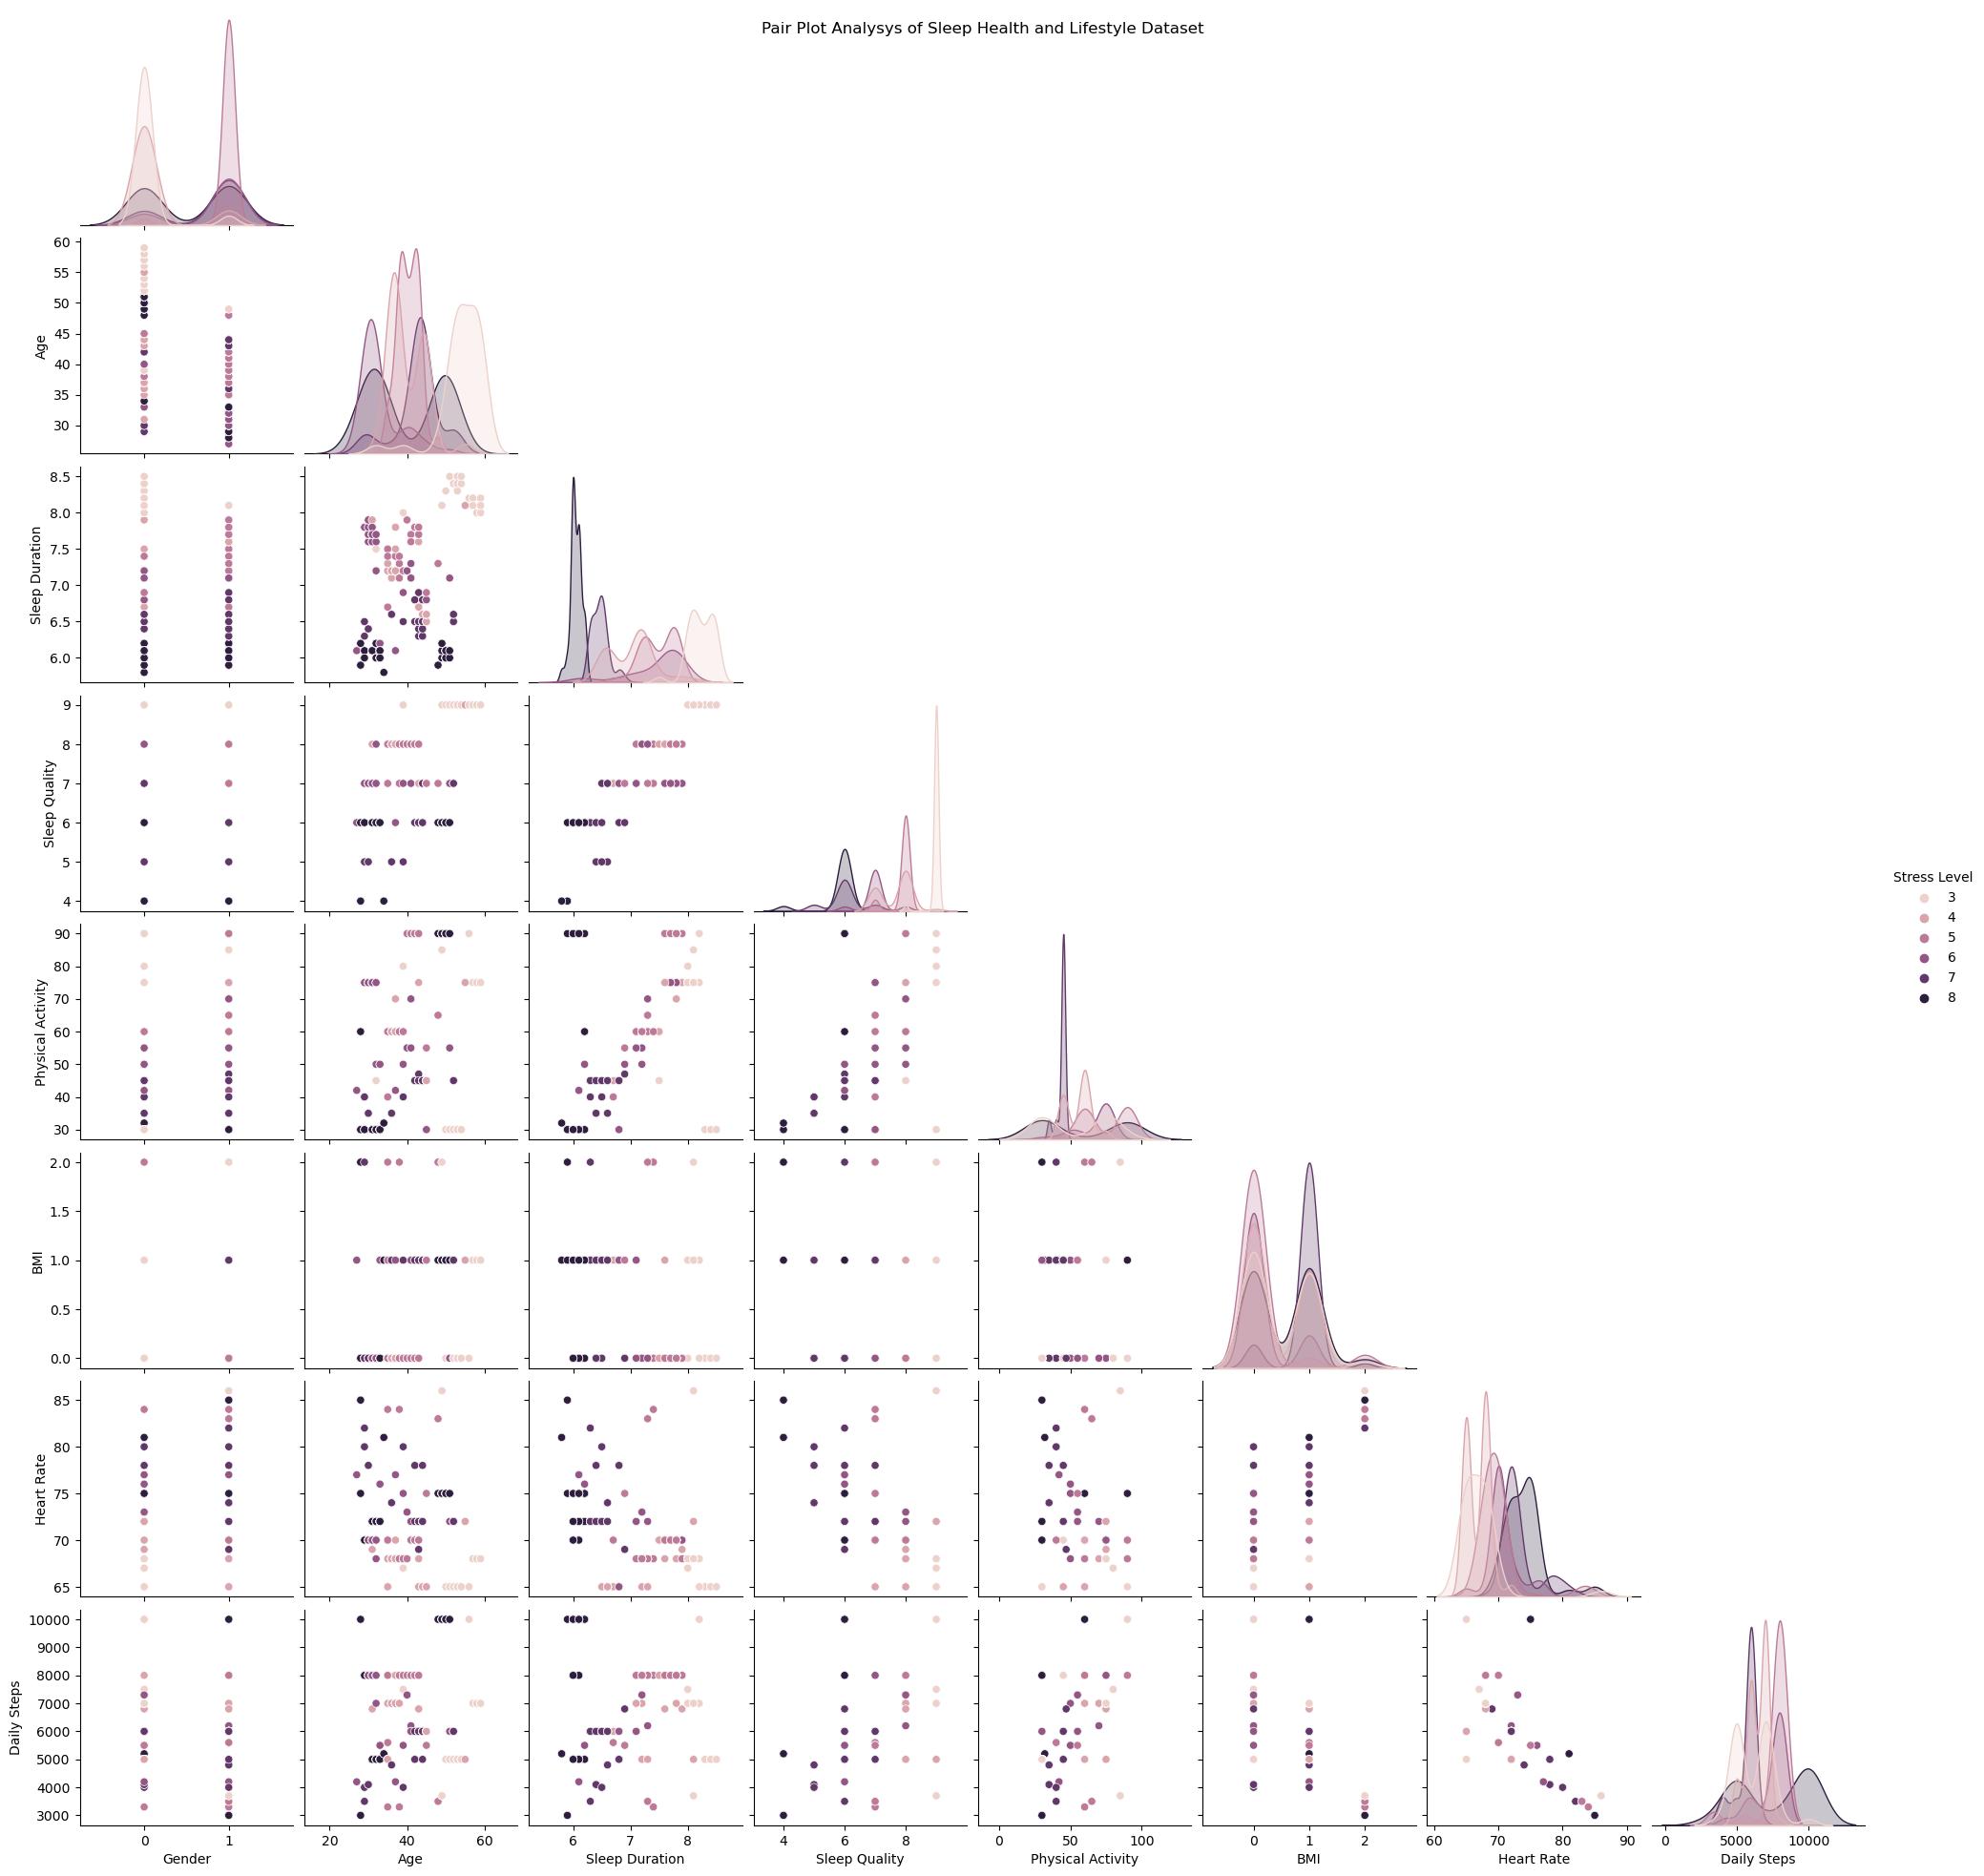
\includegraphics[width=0.75\textwidth]{pairplot.png}
        \caption{Pair Plot Matrix}
        \label{fig:pairplot}
    \end{figure}

    Subsequently, a correlation matrix (reference to figure) was constructed to examine high correlations among attributes, with a special focus on their connection to Stress Level as the dependent variable in our models. The correlation matrix reinforced the findings from the pair plot, highlighting strong negative correlations of -0.9 between Sleep Quality and Stress Level, and -0.81 between Stress Level and Sleep Duration.

    \begin{figure}[H]
        \centering
        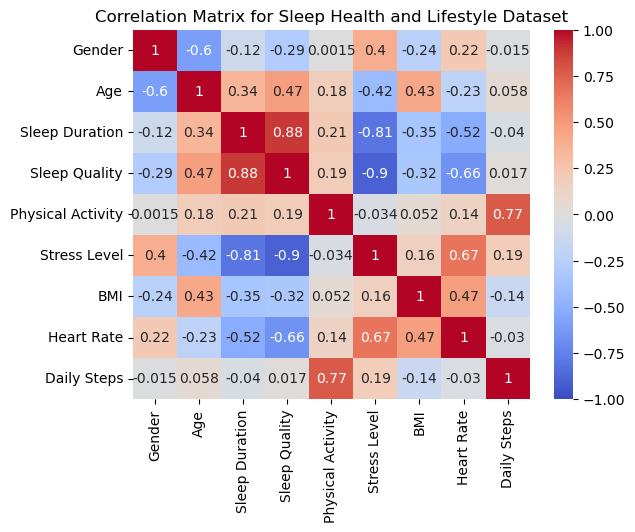
\includegraphics[width=0.75\textwidth]{correlation.png}
        \caption{Correlation Matrix}
        \label{fig:correlation}
    \end{figure}

    From these insights, it became evident that Sleep Quality and Sleep Duration were pivotal predictors of stress in our models. The potential synergistic predictive power of using these two attributes together became apparent and for that reason, we opted to use Sleep Quality and Sleep Duration as our predictors.

    We also performed some outlier detection on these important variables using box plot models. We found no significant outliers in the predictor variables or in the dependent variable Stress Level, and although Stress Level could be a value from 1 to 10, the only values for this outcome variable were between 3 and 8 from this dataset.

    \section*{Proposed Methodology}
    

    \section*{Experimental Results}

    \section*{Conclusion and Discussion}
    
    \newpage
    \section*{References}

\end{document}